\documentclass[../main/main.tex]{subfiles}

\newdate{date}{22}{10}{2020}


\begin{document}



\marginpar{ \textbf{Lecture 8.} \\  \displaydate{date}. \\ Compiled:  \today.}


\subsection{Heterogeneous Networks}

What is the effect of heterogeneity in the spread of the disease? This assumption \( k_i \sim \expval{k}  \) does not hold anymore, so we cannot assume that all the nodes are equal.

Let us consider \textbf{heteroegeneous mean-field approximation}, suppose a \textbf{ DBMF model} and let us cut the chain at an \textbf{individual level} (we consider the individual probability of getting the infection).

Let us start with the paper “Epidemic Spreading in Scale-Free Networks”. It provides a SIS model on scale-free networks.
The idea is that since nodes are not equal anymore, the probability of getting the infection strongly depends on their position (i.e. degree) in the network. The Pastor-Satorras and Vespignani's intuition is that nodes with the same degree behave in the same way.
We are gonna divide the network in degree classes: we group togheter all the nodes with the same degree.

To write down the equation we need to multiply the number of compartments:
\begin{equation*}
  s_k = \frac{S_k}{N_k}, \qquad \rho _k = \frac{I_k}{N_k}
\end{equation*}
where \( s_k \) and \( \rho _k \) are the fraction of suscpetible/infected nodes of degree \( k \) in the network. We have that \( N_k \) represent the number of nodes with degree \( k \) in the network. So, we are defined as before the number at degree \( k \) of suscpetible and infected in the system.
The total fraction of \( \rho  \) and \( s \) in the system is given by:
\begin{equation}
  \rho = \sum_{k}^{} P(k) \rho _k, \qquad s = \sum_{k}^{} P(k) s_k
\end{equation}

Now, we write the equation for each degree class:
\begin{equation}
  \dv{}{t}  \rho _k (t) = - \mu \rho _k (t) + \beta k \mathcolorbox{green!20}{(1- \rho _k (t)) \Theta _k (t)}
\end{equation}
where we have as usual a recovery and infection part.
In particular, we the probability of a contact between a suscpetible of degree \( k \) and an infected is represented in green.
The idea behind it is that we have the probability of being infected \( (1- \rho _k (t)) \) and the probability of having contact with an infected \( \Theta _k (t) \).
In particular, the probability that a node with dehree \( k \) has an infected neighbor can be expressed as:
\begin{equation}
  \Theta _k(t) = \sum_{k'}^{} P(k'|k)\rho _{k'}
\end{equation}
where we  sum over all the possibile degree classes and we are gonna see the probability of connecting with one of them, hence this is the probability that another node is infected.
Note that we are making no assumption about the function \(  P(k'|k) \) which will change with \( k \). It could be in principle anything, in the sense that it depends on the structure of the networ. However, there are some cases in which we can do some assumptions on the structure of the network.

For random networks, e.g. picking a node at random:
\begin{equation}
  P(k'|k) = \frac{k'P(k')}{\sum_{k'}^{} k' P(k')  } = \frac{k'P(k')}{\expval{k}  }
\end{equation}
where \( P(k') \) is the probability of getting a connection at random. Then, we multiply it by \( k' \) which is the number of connection that we pick up. Then we normalize over the average degree of the network.  Hence, at the end it is the probability that a point in the network points to \( k' \).  Note that \( P(k'|k) \) does not depend on \( k \).

We obtain:
\begin{equation*}
  \Theta _k (t) = \frac{\sum_{k'}^{} P(k') \rho _{k'} (t)  }{\expval{k} } = \Theta (t)
\end{equation*}
In the numerator: we take the probability that a link taken at random points to \( k' \), then we multiply by the probability of being infected and then we sum over all the possible degrees.
We note that \( \Theta _k (t) \) does not depend on \( k \) anymore. We are just picking up at random, so it should be the same for all the nodes.

The method that we are gonna use to solve the differential equation \( \dv{}{t} \rho _k (t) \) is similar to the ones used before for the other models. First of all, we assume that we are in the steady state:
\begin{equation*}
  \dv{}{t} \rho _k (t) = 0 \qquad \rightarrow  \qquad \rho _k = \frac{\beta k \Theta }{\mu + \beta k \Theta }
\end{equation*}
The next step is to substitute the expression for \( \rho _k  \) obtained inside \( \Theta  \):
\begin{equation*}
    \Theta _k (t) = \frac{\sum_{k'}^{} k' P(k') \rho _{k'} (t)  }{\expval{k} } = \Theta (t) \qquad \rightarrow \qquad \Theta = \frac{1}{\expval{k} } \sum_{k}^{} \frac{k^2 P(k) \beta \Theta }{\mu + \beta k \Theta }
\end{equation*}
this is the self consistent equation for \( \Theta  \).

The point is: if we want to solve this expression, we need some sort of trick. First of all, what happens is that as usual this expression has different solutions:
\begin{itemize}
\item the first one is the trivial solution \( \Theta =0 \), but we are interested in the non trivial one;
\item to obtain the non trivial solution let us note that:
\begin{equation*}
   \Theta = \frac{1}{\expval{k} } \sum_{k}^{} \frac{k^2 P(k) \beta \Theta }{\mu + \beta k \Theta } = f(\Theta )
\end{equation*}
Hence, the solution are the values of \( \Theta  \) equal to \( f(\Theta ) \). This is the interception between the line \( \Theta  \) and the function \( f(\Theta ) \). Since \( \Theta  \) is a probability, we have that \( 0<\Theta \le 1 \). This means that the slope of \( f(\Theta ) \) should be greater than 1.
Mathematically, it menas that:
\begin{equation*}
  \dv{}{\Theta }  \qty[ \frac{1}{\expval{k} } \sum_{k}^{} \frac{k^2 P(k) \beta \Theta }{\mu + \beta k \Theta } ]_{\Theta =0} \ge 1
\end{equation*}
leading to the condition:
\begin{equation}
\frac{\beta }{\mu \expval{k} } \sum_{k}^{}k^2 P(k) \ge 1 \qquad \rightarrow  \qquad \frac{\beta \expval{k^2} }{\mu \expval{k} } \ge 1
\end{equation}
which is the condition for an endemic state. Since the network has becoming more complex, also the structure for the condition of the endemic state is becoming complex. For the epidemic treshold:
\begin{equation}
 \frac{\beta \expval{k^2} }{\mu \expval{k} } = 1 \qquad \rightarrow \qquad \beta _c = \frac{\mu \expval{k} }{\expval{k^2} }
\end{equation}
which is pretty similar to the one found before but has a term which increase its complexity.

We have to check if it works also for an homogeneous network: this is the first check that we can make. For an homogeneous network \( \expval{k^2} = \expval{k}^2   \), recovering:
\begin{equation*}
  \beta _c = \frac{mu \expval{k} }{\expval{k^2} } = \frac{\mu }{\expval{k} }
\end{equation*}
which is exactly the expression that we saw before, so things are working well.

\end{itemize}

Recalling what we say last week, in scale-free networks with \( 2 < \gamma \le 3  \), we have \( \expval{k} \rightarrow c  \) and \( \expval{k^2}  \rightarrow \infty  \) as \( N \rightarrow \infty  \).
As the netowork is becoming larger, also its variance is becoming larger. This means that:
\begin{equation*}
  \beta _c = \frac{\mu \expval{k} }{\expval{k^2} } \rightarrow 0
\end{equation*}
so the epidemic threshold vanishes for \( N \rightarrow \infty  \).
Obviously, this is a quite important because, if our network is big enough, every disease will spread, no matter its infectivity (see Fig. \ref{fig:07_1}). When we have disease with a very low infection in a little part of population, they do not disappear because we are in a large network!
Hence, we have no more an endemic state and the epidemic threshold is really really small for most real epidemic network.
This result work as in a thermodynamic limit.

\begin{figure}[h!]
\centering
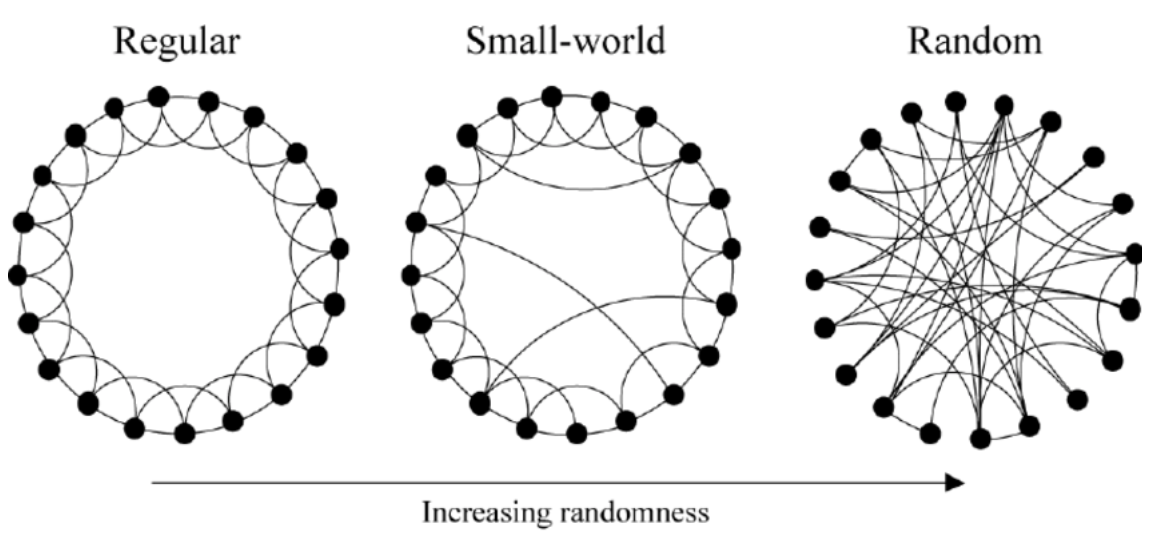
\includegraphics[width=0.6\textwidth]{../lessons/image/07/1.png}
\caption{\label{fig:07_1} In scale-free networks (and many heavy-tailed distributions) the epidemic threshold vanishes in the thermodynamic limit.}
\end{figure}

Obviously, this cannot happen in real network. What happens is that we need some finite-size correction. For example, an expression for epidemic thresold when size cannot reach infinity.
If we use scale free distribution, at some point since the degree cannot go to infinity, it is convenient to introduce an exponential cut-off.

For instance, let us consider an air trasportation network, we see that until a certain point we have a line, then the curve start to change. We cannot have an infinite number of connection. we have a line and then we will see some sort of exponential degree. The behavior is similar to the one in Fig. \ref{fig:07_2}.

\begin{figure}[h!]
\centering
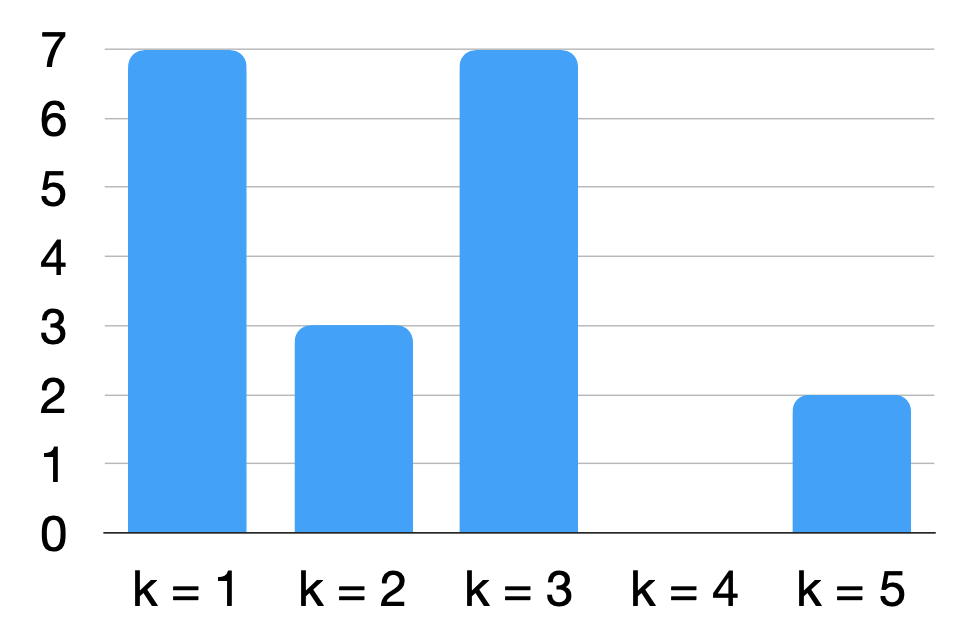
\includegraphics[width=0.7\textwidth]{../lessons/image/07/2.png}
\caption{\label{fig:07_2} Power-law with an exponential cut-off.}
\end{figure}


We can model this kind of things by adding an exponential term:
 \begin{equation}
   P(K) \sim k^{- \gamma}   e^{-k/k_c}
 \end{equation}
where \( k_c \) is a characteristic degree.
At some point the term added will becomes the dominant term. What happens? For large \( k_c \) and \( 2 < \gamma < 3  \) the epidemic threshold reads as:
\begin{equation}
  \beta _c \simeq \qty(\frac{\mu k_c}{k_{min}})^{\gamma -3 }
\end{equation}
we will not show the calculation. In the lab, we will compare the epidemic treshold in an random network and in a scale-free network to see their differences. This were the results for the SIS model in a network.






\section{SIR model in a network}

\subsection{Degree-based mean-field theories (DBMF)}

We can write the same equations for the SIR model under the same assumption of heteroegeneous mean-field.
The difference is that we need one more equation to take into account also the equation for recovered individuals. The densities are \( \rho _k^S(t) \), \( \rho _k^I (t) \) and \( \rho _k^R (t) \) with \( \rho _ \infty ^R = \lim_{t \rightarrow \infty } \sum_{k}^{} P(k) \rho _k^R (t) \). We have that:
\begin{equation}
\begin{split}
  \dv{}{t} \rho _k^I (t) &= - \mu \rho _k^I (t) + \beta k \rho _k^S (t) \Gamma _k(t)  \\
  \dv{}{t} \rho _k^R (t) &= \mu \rho _k^I (t)
\end{split}
\end{equation}
with \( \rho _k^S (t) = 1 - \rho _k^I (t) - \rho _k^R (t)\) and where:
\begin{equation}
  \Gamma _k (t) = \sum_{k'}^{} \frac{k'-1}{k'} P(k'|k) \rho _{k'}
\end{equation}
is the probability of a contact with an infected node and plays exactly the same role of \( \Theta  \) of before.
It represents the link from which the infection arrived at the node. We will not show how to obtain its form.  It is little different with respect of the SIS model because of the structure of the SIR.
There is a neibhobour that can trasmit the infection to me, but it can recover. We need to take into account that the disease is coming from one side, because that side of the network for us is forbidden in the sense that we have recovered that cannot be infected again.

The epidemic treshold for random networks results:
\begin{equation}
  \beta _c = \frac{\mu \expval{k} }{\expval{k^2} - \expval{k} }
\end{equation}
and the important things is that \( \beta _c^{SIS} \neq \beta _c^{SIR} \). This is the first time in the course that the epidemic treshold for these two models is not the same.

\subsection{Individual-based mean-field theories (IBMF)}

Before we were assuming that all the nodes with the same degree were equal. Now, we are gonna studying the individual based mean-field theories for individuals.
We are not considering a single network, but an average over all the possible network we can create given that degree distribution.
Hence, under the Heterogenous Mean-Field framework we are solving the epidemics problem for an ensemble of networks whose common feature is the \( P(k) \): ensemble of networks.


Assuming that all the nodes with the same degree are equal, we are not looking at the single network but at their average. This is what in physics is called \textbf{annealed networks}.
In the opposite when I called \textbf{quenched networks}, I am consider a particular realization of one network. The idea is: instead of considering the average we are considering a particular network. This is de difference in doing a degree bases or an indivudual based.

Let write down the equation for the quenced mean field. We are gonna use the discrete time formulation of equation because it is a bit simpler (we can write also the same things with differential equations).

We are consider \( \rho _i (t) \) as the probability of a node of being infected at time \( t \). What is my probability of being infected at time \( t+1 \) is:
\begin{equation*}
  \rho _i (t+1) = \rho _i(t) (1- \mu ) + (1 - \rho _i(t))q_i(t)
\end{equation*}
which is the probability of being infected and not get cured and the second is the normal term when I am getting the infection (the probability of being suscpetible and the probability of getting the disease).
We have that \( q_i(t) \) is the probability of node \( i \) of getting infetced by at least one neighbour.

We need an expression for \( q_i(t) \). The basic idea is that:
\begin{equation*}
  q_i (t) = 1 - \prod_{j=1}^{N} [1- \beta A_{ij} \rho _j (t)]
\end{equation*}
We have the node \( i \) in green, and the infected neighbour in red. We see that \( \beta A_{ij} \rho _j (t) \) is the probability of getting infetced by node \( j \) (at least). We have that  \( [1- \beta A_{ij} \rho _j (t)] \) is the probability of NOT getting infected by node \( j \). I have to repeat this calculation for all my infected nehbours, hence \( \prod_{j=1}^{N} [1- \beta A_{ij} \rho _j (t)] \) is the probability of NOT getting infected by any neighbor.
Finally, \(   q_i (t) \) represents the probability of getting infected by at least one neighbor.
Hence, the probability of getting infected is 1 minus the probability of not getting infected by any neighbor.

Hence, once we have this things, first of all we can solve it numerically, which means for instance by iteration. In this case we are gonna have an equation for each of the node. We have \( 2^N \) equation where \( N \) is the size of the system. The equation for \( \rho _i (t+1) \) can be solved by iteration. I am gonna repeat this equation many times until I reach the steady state.

The difference with the degree based mean field theories is that actually \( A_{ij} \) we are including all the adjiacency matrix, while before only the average.

We can also solve analytically the system at teh steady state to estimate the epidemic threshold.
I am assuming that if I am in the epidemic treshold, what happens is that \( \rho  \) is very small for all the nodes. If \( \rho _i^* = \varepsilon _i^* \ll 1 \), we can use an approximation for \( q_i^* \):
\begin{equation*}
  q_i^* = 1 - \prod_{j=1}^{N} [1- \beta A_{ij} \varepsilon _j^*] \sim \beta \sum_{j=1}^{N} A_{ij} \varepsilon _j^*
\end{equation*}
Substituting we have:
\begin{equation*}
  \mu \varepsilon _i^* = \beta (1- \varepsilon _i^*) \sum_{j=1}^{N} A_{ij} \varepsilon _{j}^*
\end{equation*}
We have a linear system where the interaction is represented by the adjiacency matrix:
\begin{equation*}
  \frac{\mu }{\beta } \varepsilon _i^* = \sum_{j=1}^{N} A_{ij} \varepsilon _j^*
\end{equation*}
This linear system has solution only if \( \frac{\mu }{\beta } \) is an eigenvalue of the adjiacency matrix \( A_{ij} \). This is why last week we say that the spectrum of the adjiacency matrix was important.
Hence:
\begin{equation*}
  \beta = \frac{\mu }{\Lambda _i}
\end{equation*}
Since, we are interested in the smallest possible value of \( \beta  \) for which we have a solution, we take the largest eigenvalue of the adjiacency matrix \( A \):
\begin{equation*}
  \beta _c = \frac{\mu }{\Lambda _{max}}
\end{equation*}
This is the expression for the epidemic treshold, and it is a general results that it is valid not only by this approxmation but for a generic case for a generic network.

What is the relation between the epidemic treshold for DBMF and IBMF?
We have that:
\begin{equation*}
  \beta _c^{DBMF} = \frac{\mu \expval{k} }{\expval{k^*} }, \qquad \beta _c^{IBMF} = \frac{\mu }{\Lambda _{max}}
\end{equation*}
The relation amogn them for scale-free networks is:
\begin{equation*}
  \Lambda _{max} \sim max(\sqrt{k_{max}}, \expval{k^*}/\expval{k}   )
\end{equation*}
Specifically:
\begin{equation*}
\beta _c \sim
  \begin{cases}
   \mu / \sqrt{k_{max}} & \gamma > 5/2  \\
   \mu \expval{k}/\expval{k^2} & 2 < \gamma < 5/2
  \end{cases}
\end{equation*}
We can conclude that IBMF is more accurate than DBMF.




\end{document}
